The dominant and sub-dominant irreducible backgrounds for~\Hllll~process are ZZ production via \qqbar annihilation and gg fusion respectively. The reducible
background is of the instrumental nature and arises from the process where partial jets are misidentified as leptons. The main processes which contributes in this 
background are: jets production in association with Z boson, jets production in association with WZ boson pair and the \TTbar pair production. From now on, this
background will be denoted as Z+X.
 \begin{table}[!hb]
\begin{center}
\caption{ The number of observed candidates, expected background and signal events passing all the selections
in the mass range of  $105 < m_{4\ell} < 140 \GeV$ utilized in the $\Hllll$ measurements. ZZ and signal events are estimated 
using MC simulations while Z+X is estimated by control regions in data.
\label{tab:EventYieldsH4l}}
\begin{tabular}{|l|c|c|c|}
\hline \hline
\textbf{Channel} & $4\Pe$ & $4\Pgm$ & $2\Pe2\Pgm$ \\
\hline \hline
\multicolumn{4}{|c|}{\usedLumiB (8 TeV)}  \\
\hline
$\Pq\Paq \to \Z\Z$ &  3.05 $\pm$  0.35  &  7.62  $\pm$  0.49  &  9.03  $\pm$  0.69 \\
\Z~+~X & 1.52 $\pm$ 0.34 & 1.18 $\pm$ 0.48 & 4.16 $\pm$ 1.06 \\
gg~$\to \Z\Z$ &  0.20  $\pm$  0.05  &  0.41  $\pm$  0.10  &  0.50  $\pm$  0.13  \\
\hline
Total background expected & 4.77 $\pm$ 0.71 & 9.21 $\pm$ 0.69 & 13.69 $\pm$ 1.29 \\
\hline
$H\rightarrow 4l$ ($m_H = 125.0$~GeV) &  2.93 $\pm$  0.45  &  5.63  $\pm$  0.67  &  7.29  $\pm$  0.93  \\
\hline
Observed  & 9 & 15 & 15 \\
\hline \hline
\multicolumn{4}{|c|}{\usedLumiA (7 TeV)}  \\
\hline
$\Pq\Paq \to \Z\Z$ &  0.84  $\pm$  0.10  &  1.80  $\pm$  0.11  &  2.24  $\pm$  0.28  \\
\Z~+~X                & 0.34 $\pm$ 0.09     & 0.22 $\pm$ 0.09     & 1.03 $\pm$ 0.29\\
$\Pg\Pg \to \Z\Z$  &  0.03  $\pm$  0.01  &  0.06  $\pm$  0.02  &  0.07  $\pm$  0.02  \\
\hline
Total background expected & 1.21 $\pm$ 0.14 & 2.08 $\pm$ 0.14 &  3.37 $\pm$ 0.40 \\
\hline
$H\rightarrow 4l$ ($m_H = 125.0$~GeV) &  0.70  $\pm$  0.11  &  1.24  $\pm$  0.14  & 1.67  $\pm$  0.26  \\
\hline
Observed  & 1 & 3 & 6 \\
\hline \hline
\end{tabular}
\end{center}
\end{table}
\par
The irreducible backgrounds  $\Pq\Paq \to \Z\Z$ and gg~$\to \Z\Z$ for $\Hllll$ integrated and differential measurements are estimated from  Monte Carlo (MC) 
simulation as done earlier in Ref.~\cite{Chatrchyan:2013mxa}. In addition, following the study in Ref.~\cite{Bonvini:2013}, in these measurements we have
increased the expected yield for the gg~$\to \Z\Z$ background by assigning to the leading order (LO) background cross section a $m_{4\ell}$ dependent k-factor
equal to the one used for the signal $\Hllll$ process. In the region ($105 < m_{4\ell} < 140 \GeV$) this factor leads to an increase of the expected
 gg~$\to~ZZ$ background by a factor of $\sim 2.66$. After the inclusion of this k-factor, the gg~$\to ZZ$ process is still a sub-dominant 
 background in all $\Hllll$ measurements.
 \par  
 The reducible background (Z+X) is evaluated using a tight-to-loose ``fake rate'' method and the control regions in
the data, following Ref.~\cite{Chatrchyan:2013mxa}. The yields of the Z+X background are determined by two methods 
( opposite sign (OS) or same sign (SS)) are found to be consistent  with each within statistical uncertainties. 
The first control region is obtained by requiring that two leptons passing loose selections which does fulfill the criteria of $\Z_1$ candidate (failing ID and 
isolation requirements), while the other two leptons in the event passes  the criteria of $\Z_1$ candidate.  The sample is represented as 
"2 Prompt + 2 Fail`` (2P2F) sample. This sample is populated  with the events contains only two prompt leptons (mostly Drell-Yan with small fraction of
$\Zgam$ and $\TTbar$ events). The second control region is obtained by requiring that three leptons pass the final requirements. The sample is represented as 
"3 Prompt + 1 Fail`` (3P1F) sample.
\par 
The $m_{4\ell}$ shape of the reducible background is attained from OS method by performing a fit of $m_{4\ell}$ distributions of 3P1F and 2P2F  events
independently by empirical analytical functional constructed by Landau~\cite{landau:1944} in Ref.~\cite{Chatrchyan:2013mxa}.
Prediction for the reducible background in all three channels together fitted  using this empirical shape with indicated total uncertainty is shown in 
Figure~\ref{fig:ZX}. In case of the differential $\Hllll$ measurements, the shape of the
reducible background is obtained from the templates built from the control regions in data for each bin of the observable considered for the measurement,
following a procedure similar to the one used in the spin-parity studies described in the Ref.~\cite{Chatrchyan:2013mxa}.
More details on this procedure and template shapes for each of the differential $\Hllll$ measurements will be given in Section \ref{sec:ExtractionDifferential}.
\par 
The number of estimated signal and background events, along with observed data events passing all selections in the mass range used for 
$\Hllll$ measurements ($105 < m_{4\ell} < 140 \GeV$) are listed in Table~\ref{tab:EventYieldsH4l} for 7 and 8~TeV. 
\par 
Figure~\ref{fig:mass4l} shows the reconstructed four-leptons invariant mass distribution for whole 7 and 8~TeV data and MC samples 
in mass range ($50 < m_{4\ell} < 140 \GeV$) covering both  $\Hllll$ and $\Zllll$ measurements range. Predictions for the reducible background in a
wide range of $m_{4\ell}$ in all three channels
together, fitted using the empirical shape with indicated total uncertainty, is separately shown in Figure~\ref{fig:ZX}.
% 

%============
\begin{figure}[!htbp]
\begin{minipage}{0.5\linewidth}
\centerline{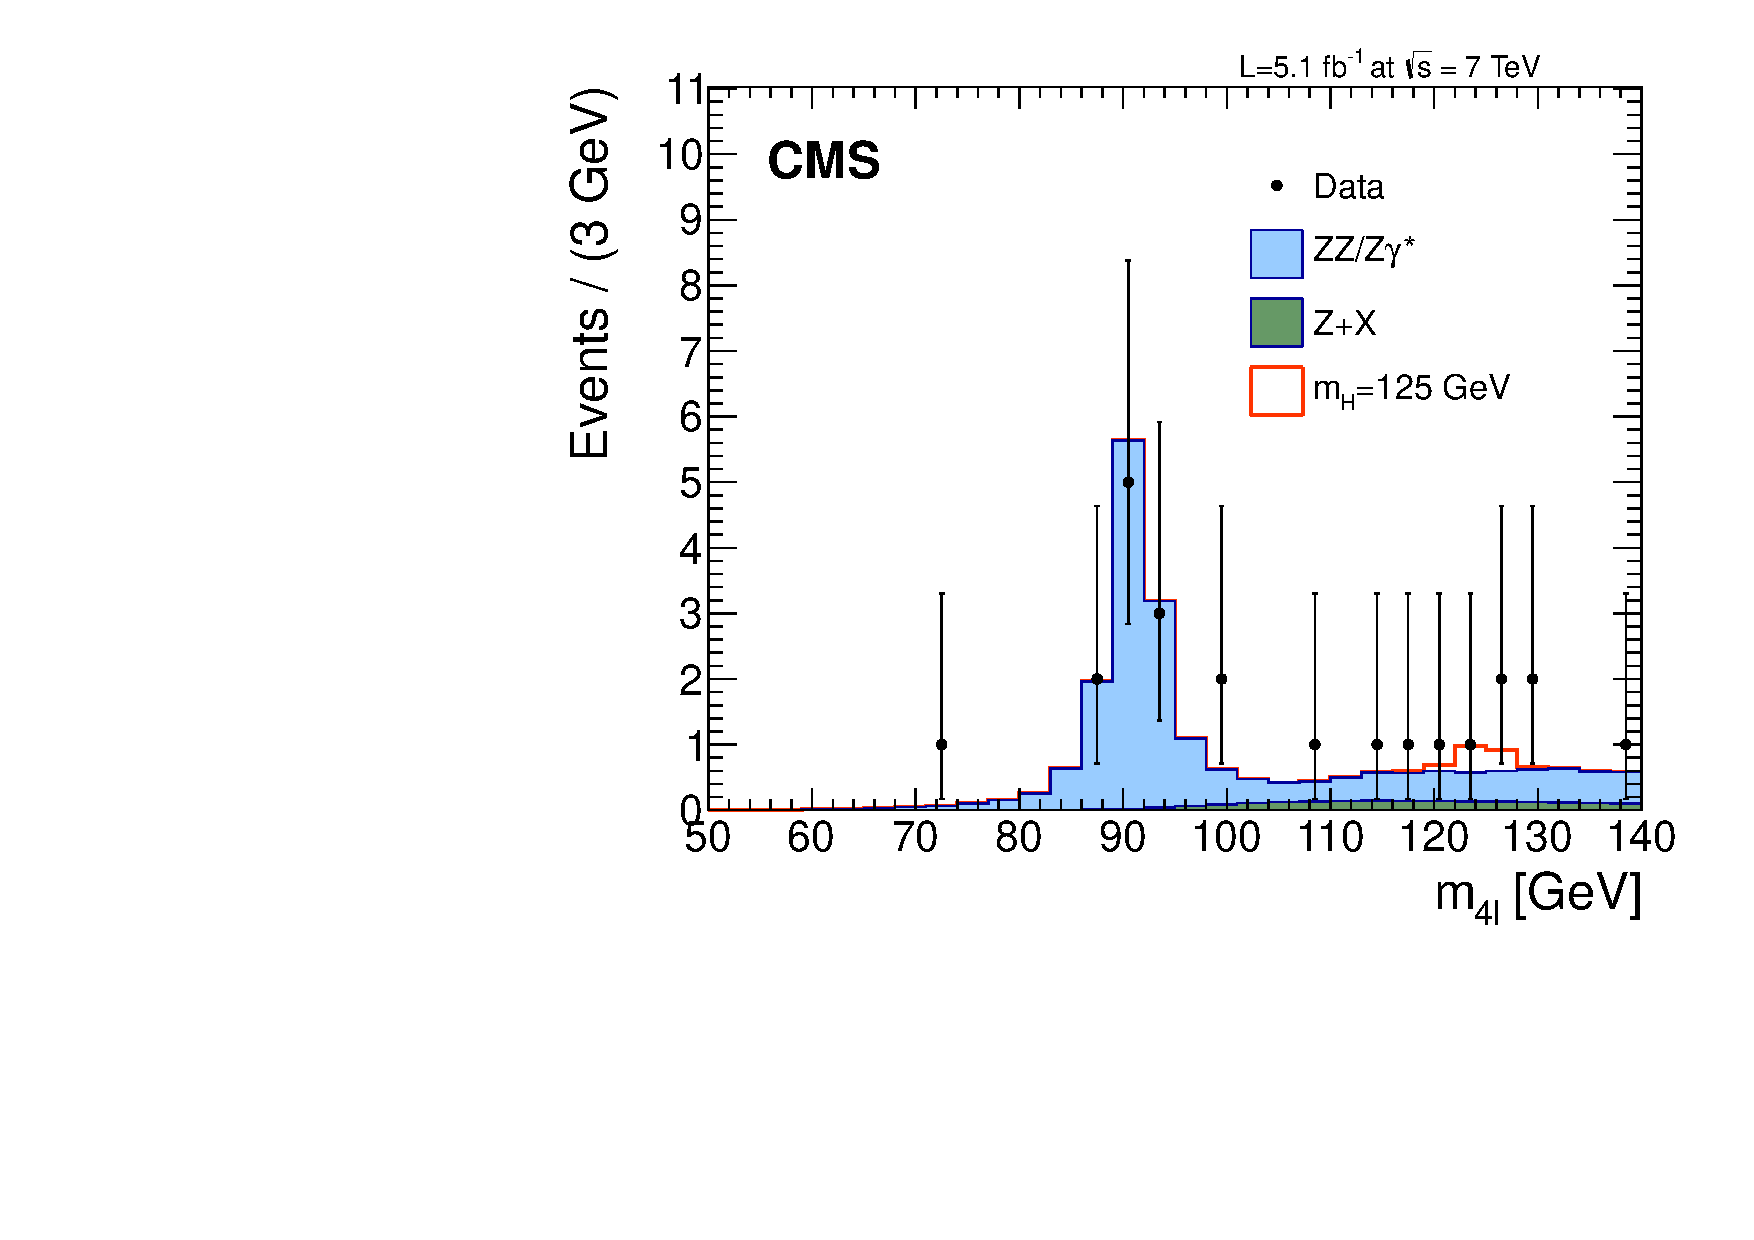
\includegraphics [width=\linewidth] {Chapters/Chapter4/AnalysisStrategy/figures/Mass4l_DataMC_7TeV_mH125GeV_fullRange.pdf}}
\end{minipage}
\begin{minipage}{0.5\linewidth}
\centerline{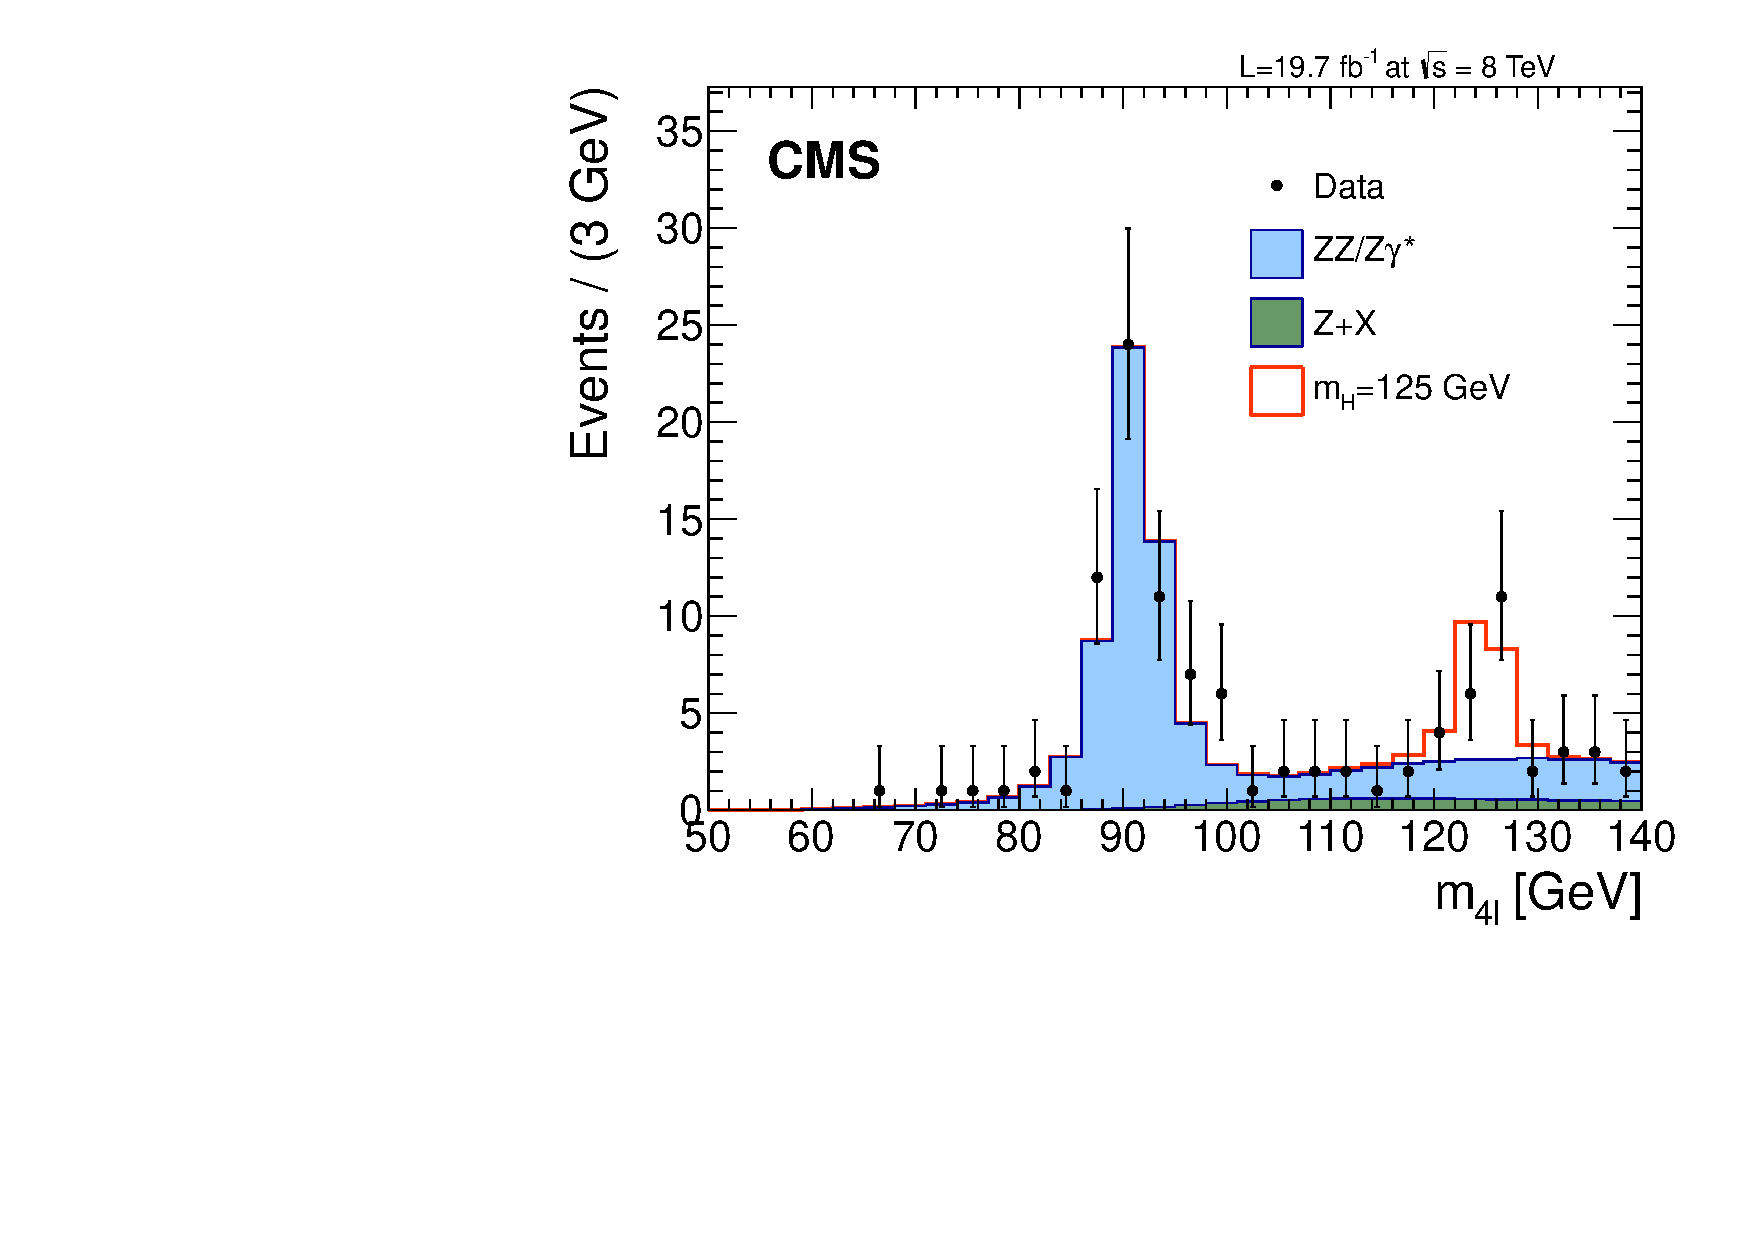
\includegraphics [width=\linewidth] {Chapters/Chapter4/AnalysisStrategy/figures/Mass4l_DataMC_8TeV_mH125GeV_fullRange.pdf}}
\end{minipage}
\caption{ Distributions of invariant mass of four-leptons using  7~TeV (left) and 8~TeV (right) datasets, along with predictions for Standard Model Higgs
          ($m_H=125.0$ GeV), including $Z\rightarrow4\ell$ resonance.}
\label{fig:mass4l}
\end{figure}

%=============

 \begin{figure}[!htbp]
 \begin{center}
   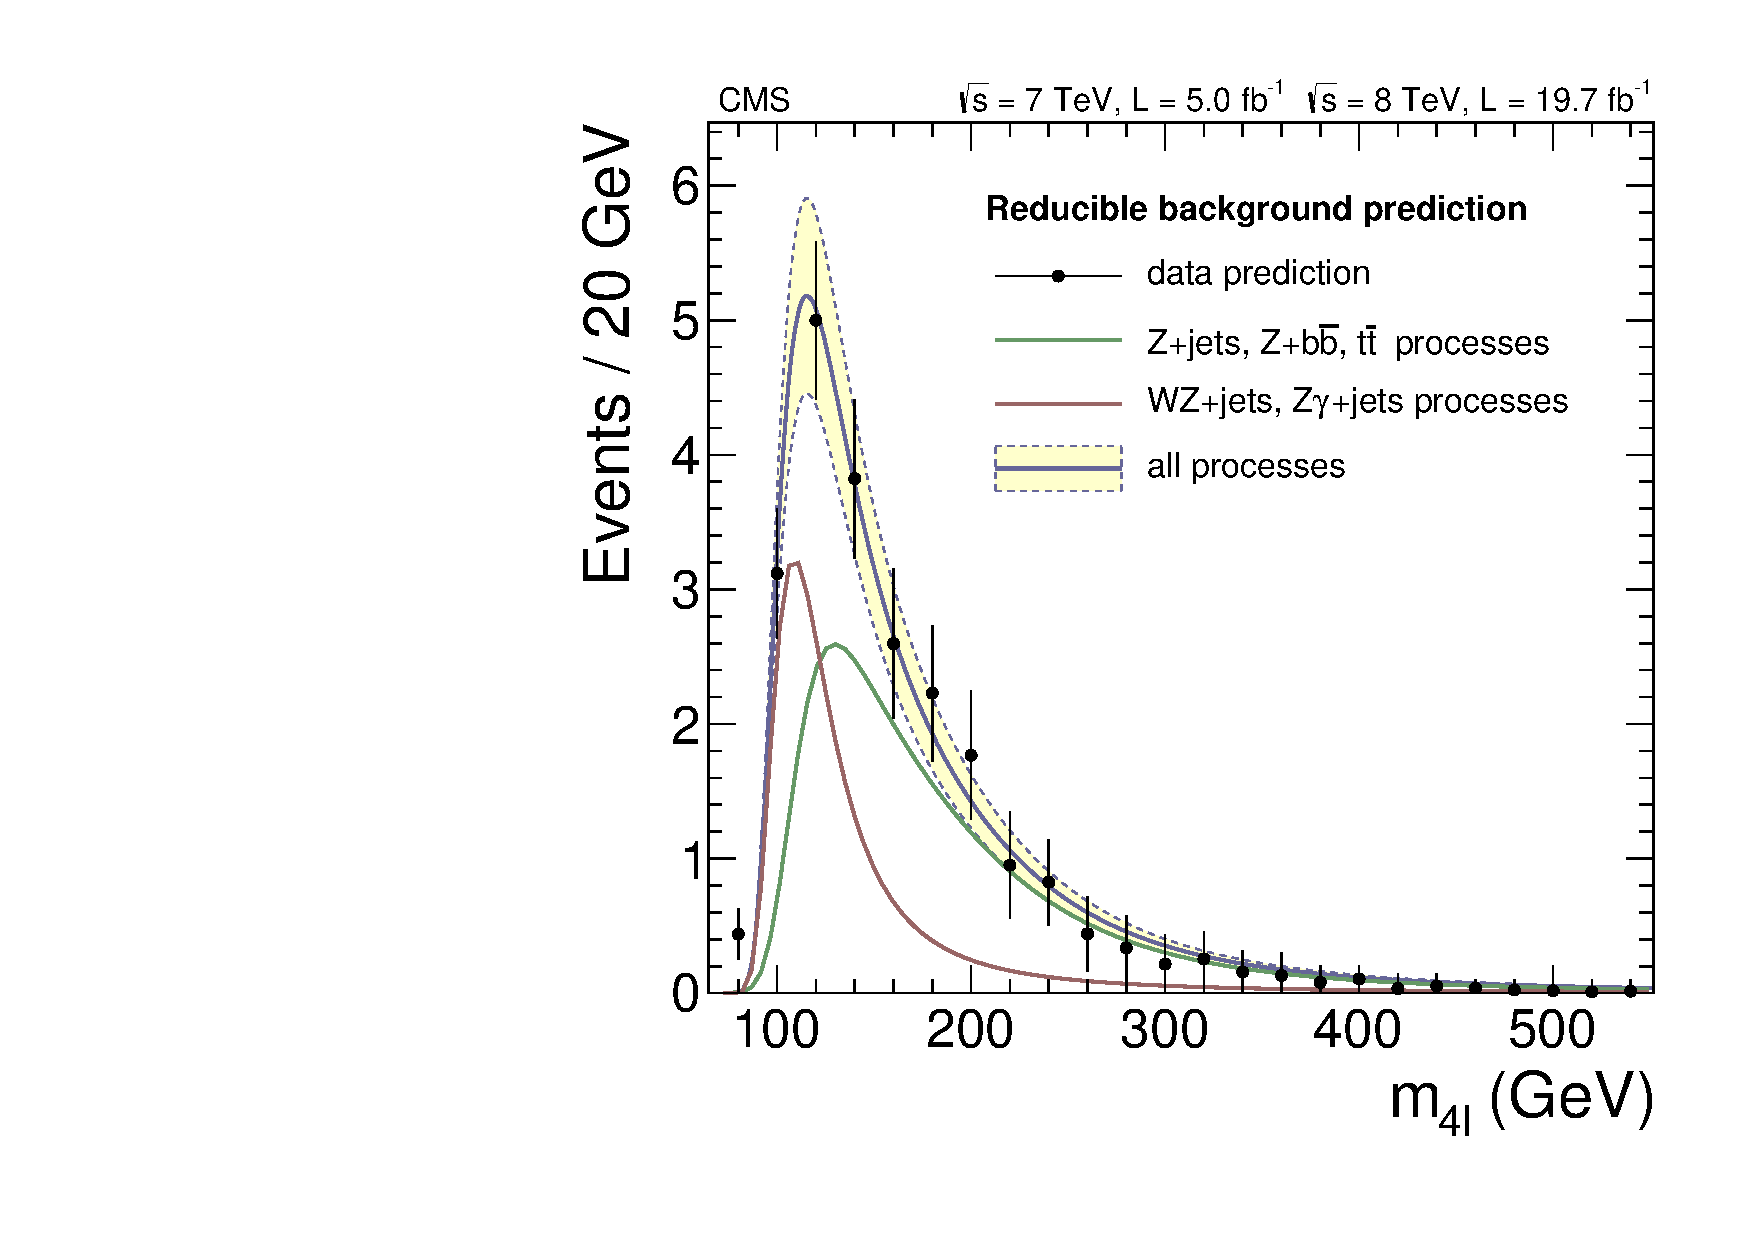
\includegraphics[width=0.60\textwidth]{Chapters/Chapter4/AnalysisStrategy/figures/RedBkgPrediction_A.pdf}
   \caption{Prediction for the reducible background in all three channels together (black dots) fitted using an empirical shape (blue curve) with 
   indicated total uncertainty (yellow band). Contributions from the 2P2F-like (green) and 3P1F-like (red) processes are fitted separately.}
 \label{fig:ZX}
 \end{center}
 \end{figure}
%============
